\section{Data Taking}
\label{sec:data taking}

The results reported here are based on data taken in September 2016 during a sequence of dedicated LHC proton fills (5313, 5314, 5317 and 5321) with the special beam properties described in the previous section.

% paragraph below: numbers taken from RunLog, bunching schemes
%   singla_6b_4_0_0_1bpi_6inj (5313), singla_6b_5_0_0_1bpi_6inj (5314 and 5317), singla_6b_5_0_0_1bpi_6inj_alt (5321
The vertical RPs approached the beam centre to only about 3 times the beam width, $\sigma_{y}$, resulting in an acceptance for $|t|$-values down to $8 \times 10^{-4}\,\rm GeV^{2}$. The exceptionally close distance was possible due to the low beam intensity in this special beam operation: each beam contained only four or five colliding bunches and one non-colliding bunch for background monitoring, each with about $2\times 10^{11}$ protons.

A similar collimation strategy as in \cite{totem-1km} was applied to keep the beam halo background under control. As a first step, vertical collimators TCLA scraped the beam down to $2\,\sigma_{y}$, then the collimators were retracted to $2.5\,\sigma_{y}$, thus creating a $0.5\,\sigma_{y}$ gap between the beam edge and the collimator jaws. A similar procedure was performed in the horizontal plane: collimators TCP.C scraped the beam to $3\un{\sigma_{x}}$ and then were retracted to $5.5\un{\sigma_{x}}$, creating a $2.5\un{\sigma_x}$ gap. With the halo strongly suppressed and no collimator producing showers by touching the beam, the RPs at $3\,\sigma_{y}$ were operated in a background-depleted environment for about one hour until the beam-to-collimator gap was refilled by diffusion, as diagnosed by the increasing shower rate (red graph in Figure~\ref{fig:rates_vs_time}). When the background conditions had deteriorated to an unacceptable level, the beam cleaning procedure was repeated, again followed by a quiet data-taking period.

% TODO: typical values for sigma_y and sigma_x

% TODO: typical instataneous luminosity

% TODO: introduce the diagonals

The horizontal RPs were only needed for the data-based alignment and therefore placed at a safe distance of $8\,\sigma_{x} \approx 5$\,mm, close enough to have an overlap with the vertical RPs (Figure~\ref{fig:rpsketch}, right).

\begin{figure*}
\begin{center}
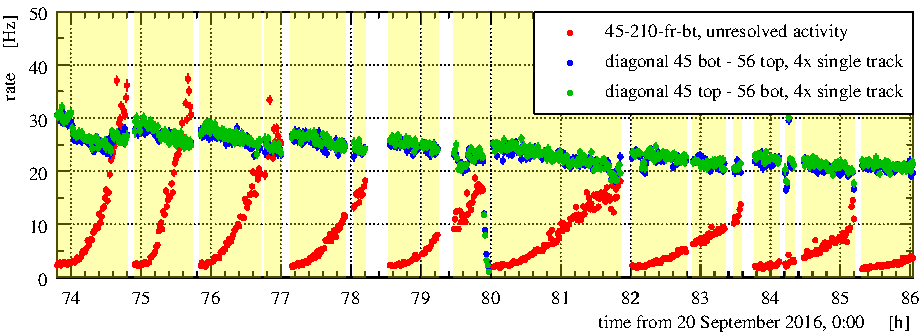
\includegraphics{fig/rates_vs_time.pdf}
%\vskip-3mm
\caption{%
Event rates from run 5321 as a function of time. The blue and green graphs give rates of fully reconstructed events in the two diagonal configurations relevant for elastic scattering. The red graph shows a rate of high-multiplicity events in a single RP (45-210-nr-hr) where no track can be reconstructed.
}
\label{fig:rates_vs_time}
\end{center}
\end{figure*}

The events collected were triggered by a logical \textit{OR} of: double-arm proton trigger 
(coincidence of any RP left of IP5 and any RP right of IP5) and zero-bias trigger (random bunch crossings) for calibration purposes.

In total, an integrated luminosity of $0.4\,\rm nb^{-1}$ % TODO: this is a crude estimate, try getting a better one from TOTEM data
was accumulated in which more than 7 millions of elastic event candidates were tagged.
